% When using TeXShop on the Mac, let it know the root document. The following must be one of the first 20 lines.
% !TEX root = ../design.tex

% Licensed to the Apache Software Foundation (ASF) under one
% or more contributor license agreements.  See the NOTICE file
% distributed with this work for additional information
% regarding copyright ownership.  The ASF licenses this file
% to you under the Apache License, Version 2.0 (the
% "License"); you may not use this file except in compliance
% with the License.  You may obtain a copy of the License at

%   http://www.apache.org/licenses/LICENSE-2.0

% Unless required by applicable law or agreed to in writing,
% software distributed under the License is distributed on an
% "AS IS" BASIS, WITHOUT WARRANTIES OR CONDITIONS OF ANY
% KIND, either express or implied.  See the License for the
% specific language governing permissions and limitations
% under the License.

\chapter[Graph]{Graph}

\begin{moduleinfo}
\item[Author] \href{mailto:okislal@pivotal.io}{Orhan Kislal}
\item[History]
	\begin{modulehistory}
		\item[v0.1] Initial version, SSSP only.
		\item[v0.2] Graph Framework, SSSP implementation details.
	\end{modulehistory}
\end{moduleinfo}


% Abstract. What is the problem we want to solve?

This module implements various graph algorithms that are used in a number of applications such as social networks, telecommunications and road networks.

\section{Graph Framework} \label{sec:graph:fw}

MADlib graph representation depends on two structures, a \emph{vertex} table and an \emph{edge} table. The vertex table has to have a column of vertex ids. The edge table has to have 2 columns: source vertex id, destination vertex id. For most algorithms an edge weight column is required as well. The representation assumes a directed graph, an edge from $x$ to $y$ does \emph{not} guarantee the existence of an edge from $y$ to $x$. Both of the tables may have additional columns as required. Multi-edges (multiple edges from a vertex to the same destination) and loops (edge from a vertex to itself) are allowed. For ideal performance, vertex and edge tables should be distributed on vertex id and source id respectively. This representation does not impose any ordering of vertices or edges. An example graph is given in Figure~\ref{sssp:example} and its representative tables are given in Table~\ref{sssp:rep}.

\begin{figure}[h]
	\centering
	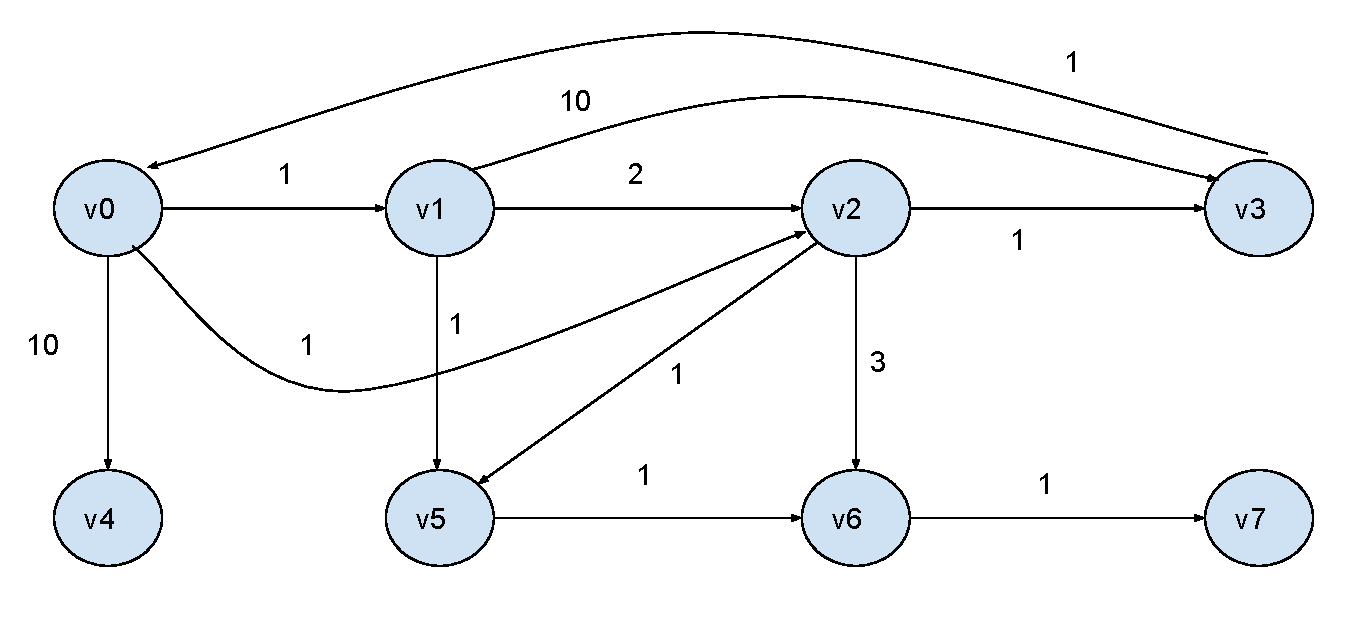
\includegraphics[width=0.9\textwidth]{figures/graph_example.pdf}
\caption{A sample graph}
\label{sssp:example}
\end{figure}

\begin{table}
  \begin{tabular}{| c | }
    \hline
    vid \\ \hline
    0 \\ \hline
    1 \\ \hline
    2 \\ \hline
    3 \\ \hline
    4 \\ \hline
    5 \\ \hline
    6 \\ \hline
    7 \\
    \hline
  \end{tabular}
  \quad
  \begin{tabular}{| c | c | c |}
    \hline
    src & dest & weight \\ \hline
    0 & 1 & 1 \\ \hline
    0 & 2 & 1 \\ \hline
    0 & 4 & 10 \\ \hline
    1 & 2 & 2 \\ \hline
    1 & 3 & 10 \\ \hline
    1 & 5 & 1 \\ \hline
    2 & 3 & 1 \\ \hline
    2 & 5 & 1 \\ \hline
    2 & 6 & 3 \\ \hline
    3 & 0 & 1 \\ \hline
    5 & 6 & 1 \\ \hline
    6 & 7 & 1 \\
    \hline
  \end{tabular}
  \caption{Graph representation of vertices (left) and edges(right) in the database}
  \label{sssp:rep}
\end{table}


\section{Single Source Shortest Path} \label{sec:graph:sssp}

Given a graph and a source vertex, single source shortest path (SSSP) algorithm finds a path for every vertex such that the sum of the weights of its constituent edges is minimized.

Shortest path is defined as follows. Let $e_{i,j}$ be the edge from vertex $i$ to vertex $j$ and $w_{i,j}$ be its weight. Given a graph G, the shortest path from $s$ to $d$ is $P = (v_1, v_2 \dots, v_n)$ (where $v_1=s$ and $v_n=d$) that over all possible $n$ minimizes the sum $ \sum _{i=1}^{n-1}f(e_{i,i+1})$.

% \subsection{Bellman Ford Algorithm}

Bellman-Ford Algorithm \cite{bellman1958routing,ford1956network} is based on the following idea: We start with a naive approximation for the cost of reaching every vertex. At each iteration, these values are refined based on the edge list and the existing approximations. If there are no refinements at any given step, the algorithm returns the calculated results. If the algorithm does not converge in $|V|-1$ iterations, this indicates the existence of a negative cycle in the graph.


\begin{algorithm}[SSSP$(V,E,start)$] \label{alg:sssp}
\alginput{Vertex set $v$, edge set $E$, starting vertex $start$}
\algoutput{Distance and parent set for every vertex $cur$}
\begin{algorithmic}[1]
	\State $toupdate(0) \set (start,0,start)$
	\For{every $i \in 0\dots|V|-1$}
		\For{every tuple $t \in toupdate(i)$} \label{alg:sssp:update}
			\For{every edge $e \mid e.src = t.id$}
		 		\State $local \set e.val + t.val$
		 		\If{$local < toupdate(i+1,e.dest).val$} \label{alg:sssp:single}
		 			\State $toupdate(i+1,dest) \set (local,e.src)$
		 		\EndIf
			\EndFor
		\EndFor
		\For{every tuple $t \in toupdate(i+1)$}
		 	\If{$t.val < cur(t.id).val$}
		 		\State $cur(t.id) \set (t.val,t.parent)$
		 	\EndIf
		\EndFor
	\EndFor
\end{algorithmic}
\end{algorithm}

\begin{description}
\item edge: (src,dest,val). The edges of the graph.
\item cur: id -> (val,parent). The intermediate SSSP results.
\item toupdate: iter -> (id -> (val,parent)). The set of updates.
\end{description}

Changes from the standard Bellman-Ford algorithm:

\begin{description}
\item Line~\ref{alg:sssp:update}: We only check the vertices that have been updated in the last iteration.
\item Line~\ref{alg:sssp:single}: At each iteration, we update a given vertex only one time. This means the toupdate set cannot contain multiple records for the same vertex which requires the comparison with the existing value.
\end{description}

This is not a 1-to-1 pseudocode for the implementation since we don't compare the `toupdate` table records one by one but calculate the overall minimum. In addition, the comparison with `cur` values take place earlier to reduce the number of tuples in the `toupdate` table.

\subsection{Implementation Details}

In this section, we discuss the MADlib implementation of the SSSP algorithm in depth.

\begin{algorithm}[SSSP$(V,E,start)$] \label{alg:sssp:high}
\begin{algorithmic}[1]
	\Repeat
		\State Find Updates
		\State Apply updates to the output table
	\Until {There are no updates}
\end{algorithmic}
\end{algorithm}

The implementation consists of two SQL blocks that are called sequentially inside a loop. We will follow the example graph at Figure~\ref{sssp:example} with the starting point as $v_0$. The very first update on the output table is the source vertex. Its weight is $0$ and its parent is itself ($v_0$). After this initialization step, the loop starts with Find Updates (the individual updates will be represented with <dest,value,parent> format). Looking at the example, it is clear that the updates should be <1,1,0>, <2,1,0> and <4,10,0>. We will assume this iteration is already completed and look how the next iteration of the algorithm works to explain the implementation details.

\begin{algorithm}[Find Updates$(E,old\_update,out\_table)$]
\label{alg:sssp:findu}
\begin{lstlisting}
INSERT INTO new_update
	SELECT DISTINCT ON (y.id) y.id AS id,
		y.val AS val,
		y.parent AS parent
	FROM out_table INNER JOIN (
			SELECT edge_table.dest AS id, x.val AS val, old_update.id AS parent
			FROM old_update
				INNER JOIN edge_table
				ON (edge_table.src = old_update.id)
				INNER JOIN (
					SELECT edge_table.dest AS id,
						min(old_update.val + edge_table.weight) AS val
					FROM old_update INNER JOIN
						edge_table AS edge_table ON
						(edge_table.src=old_update.id)
					GROUP BY edge_table.dest
				) x
				ON (edge_table.dest = x.id)
			WHERE ABS(old_update.val + edge_table.weight - x.val) < EPSILON
		) AS y ON (y.id = out_table.vertex_id)
	WHERE y.val<out_table.weight
\end{lstlisting}
\end{algorithm}

We begin our analysis of Find Updates function from its innermost subquery. This subquery (lines 11-16) takes a set of vertices (in the table $old\_update$) and finds the reachable vertices. In case a vertex is reachable by multiple vertices, only the path that has the minimum cost is considered. This means the input vertices need the value of their path as well. In our example, both $v_1$ and $v_2$ can reach $v_3$. In this case, we would have to use $v_2$ -> $v_3$ edge since that gives the lowest possible path value. Please note that we are aggregating the rows using the $min$ operator for each destination vertex and we are unable to return the source vertex at the same time. This means we know the value of $v_3$ should be $2$ but we cannot know its parent ($v_2$) at the same time. To solve this limitation, we combine the result with $edge$ and $old\_update$ tables (lines 7-10) and get the rows that has the same minimum value. At this point, we would have to tackle the problem of tie-breaking. Vertex $v_5$ has two paths leading into: <5,2,1> and <5,2,2>. The inner subquery will return <5,2> and it will match both of these edges. However, it is redundant to keep both of them in the update list as that would require updating the same vertex multiple times in a given iteration. By using the $DISTINCT$ clause at line 2, we allow the underlying system to accept only a single one of them. Finally, we want to make sure these updates are actually leading us to shortest paths. Line 21 ensures that the values stored in the $out\_table$ does not increase and the solution does not regress throughout the iterations.

Applying updates is straightforward as the values and the associated parent values are replaced using the $new\_update$ table. After this operation is completed the $new\_update$ table becomes $old\_update$ for the next iteration of the algorithm.

